\section{Deep Learning for Inference}

\subsection{Revision of Deep Learning}
Deep learning is a rapidly developing field within machine learning that recently got a lot of attention within economics.
The idea is to take complex data and to represent it by a series of simpler representations, each of which is expressed in terms of the previous one \citep{Goodfellow-et-al-2016}.
A common example of this is the \textit{feedforward neural network}, which is a series of layers of neurons, each of which is connected to the next layer.
The first layer is the input layer, the last layer is the output layer, and the layers in between are called hidden layers.
The input layer corresponds to the covariates $X$, the output layer corresponds to the outcome $Y$.
Figure \ref{fig:1} illustrates the layer and node structure of a \ac{mlp}, which is a special class of feed forward networks and is commonly used in empirical applications \citep{farrellDeepNeuralNetworks2021}.
From hence on I use \ac{mlp} and deep learning interchangeably as it is the approach used in this paper.

\begin{figure}%                 use [hb] only if necceccary!
\centering
\caption{Illustration of a feedforward neural network \citep{farrellDeepNeuralNetworks2021}}
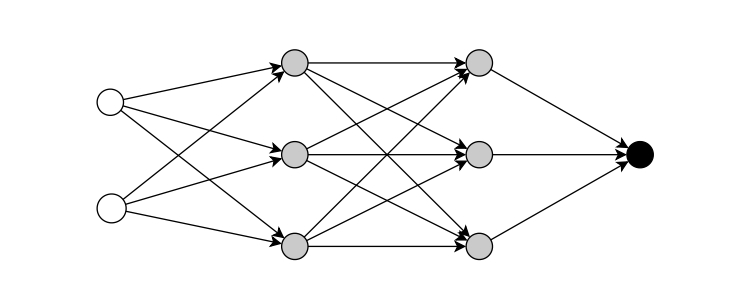
\includegraphics[width=\textwidth]{Neural_net}
\caption*{\textbf{Note:} This figure illustrates the basic structure of a \ac{mlp} $\mathcal{F}_{\text{MLP}}$, showing the input layer with $d=2$ neurons in white. The two ($H=2$) hidden layers in grey with $U=6$ neurons, and one output layer in black ($L=1$). The total amount of weights is $W=28$.}
\label{fig:1}
\end{figure}

The actual computation within the neural networks is done by the \textit{activation function} $ \sigma : \mathbb{R} \to \mathbb{R} $, which is applied to the output of each hidden neuron.
The most common activation function is the \ac{relu} function, which is defined as $ \sigma(x) = \max(0, x) $ and used in this thesis.
The advantage of the linear \ac{relu} is that it is computationally fast and the circumvents the vanishing gradient problem, which is a common problem in deep learning.\footnote[1]{The vanishing gradient issue arises especially by activation functions like \textit{sigmoid} and \textit{tanh}.
When the neural network model is trained, all the weights of the model are updated through a process called \textit{backpropagation}.
Backpropagation is the algorithm used to compute the gradient of the loss function with respect to each parameter, which is then used to update the parameters in the direction that minimizes the loss.
The issue that can arise is that updating of parameters is hindered or training is completely stopped \citep{abuqaddom2021oriented}.}
\ac{relu} takes any linear combination given by $\tilde{x}' w + b$ and transforms it to $ \sigma(\tilde{x}' w + b)$, where $w$ is the weight vector, $b$ is the constant term\footnote[2]{The actual term in computer science is \textit{bias} but to reduce confusion with the inference use of the term I follow \citet{farrellDeepNeuralNetworks2021} and use the term \textit{constant} as well.}, and $\tilde{x}$ is the input vector.
One can clearly see that the \ac{relu} sets all negative values from the linear combination $\tilde{x}' w + b$ to zero, while keeping all positive values unchanged.
%dont do the footnote write that out here

The main problem the neural network wants to solve is to estimate the unknown function $f^*(x)$.
More precisely, $f^*$ is a function that maps the input $\tilde{x}$ to the output $\tilde{y}$.
As $f^*$ is unknown, the neural network tries to estimate it by minimizing the expected loss function $\mathbb{E}[\ell(f, Z)]$, such that one can write:
\begin{equation}
f^* = \arg \min_f \mathbb{E}[\ell(f, Z)],
\end{equation}
where $\ell(f, Z)$ is the loss function, which is a measure of how well the model is performing. %change it here
The loss function can be represented by many different function such as least squares or logistic regression, where the latter one is used in this thesis.
\begin{equation}
f^*(x) := \log \left( \frac{\mathbb{E}[Y|X = x]}{1 - \mathbb{E}[Y|X = x]} \right) \quad \text{and} \quad \ell(f, z) = -yf(x) + \log(1 + e^{f(x)}). \quad \text{(2.3)}
\end{equation}

\subsection{Deep Learning for Difference in Differences}
